\section{Simple Operations on Signals}
%-----------------Transformations of the Time Variable--------------------%
 \subsection{Transformations of the Time Variable}
 \begin{itemize}
 \item Time delay
 \item Time reversal 
 \item Time scaling
 \end{itemize}
\begin{figure}[H]
    \centering 
    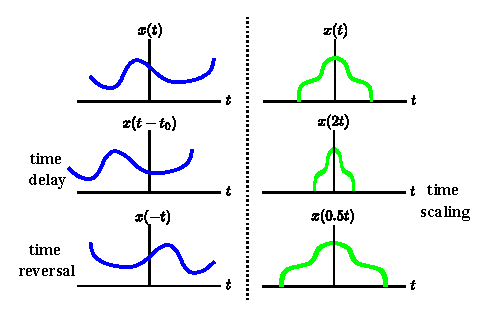
\includegraphics[width=.7\textwidth]{images/transformation.eps}
    \caption{Transformations applies to the time variable: time delay (left middle), time reversal (left bottom), time scaling (right)} 
\end{figure}
%-----------------Amplitude Transformation--------------------%
  \subsection{Amplitude Transformation}
  \[ y(x) = Ax(t)+B \]
  \quad where $A,B$ are constants.
%-----------------Linear Combination--------------------%
\subsection{Linear Combination}
\begin{itemize}
\item In continuous-time domain:
\[ y(t) = a_{1}x_{1}(t)+a_{2}x_{2}(t)+...+a_{N}x_{N}(t) \]
\item In discrete-time domain:
\[ y[n] = a_{1}x_{1}[n]+a_{2}x_{2}[n]+...+a_{N}x_{N}[n] \]
 \quad where $a_{i} \in \mathbb{C}$, $i=1,2,...,N$ are real or complex numbers.
\end{itemize}
%-----------------Multiplication--------------------%
\subsection{Multiplication} 
\begin{itemize}
\item In continuous-time domain: 
\[ y(t) = x_{1}(t) \cdot x_{2}(t) \]
\item In discrete-time domain:
\[ y[n] = x_{1}[n] \cdot x_{2}[n] \]
\end{itemize}
This implies \textbf{instantaneous multiplication} for each time instant or each discrete time sample.
%-----------------Scaler product and norm--------------------%
\subsection{Scalar Products and Norms}
%-----------------Scaler product and norm of vectors--------------------%
\subsubsection{Scalar Product and Norm of Vectors}
\begin{itemize}
\item The \textbf{scalar product} between two 3-D vectors $\vec{A}$ and $\vec{B}$: projection of $\vec{A}$ on $\vec{B}$.
\[ \vec{A} \cdot \vec{B} = A_{x} \cdot B_{x} + A_{y} \cdot B_{y} + A_{z} \cdot B_{z} = \lvert \vec{A} \rvert \cdot \lvert \vec{B} \lvert \cos(\phi) \]
%The \textbf{scaler} product between the 3D vectors $\vec{A}$ and $\vec{B}$ is computed as the sum of the multiplication between entries $(A_{x} \cdot B_{x} + A_{y} \cdot B_{y} + A_{z} \cdot B_{z})$, or equivalently as $A\cdot B \cos(\phi)$, where $A$ and $B$ is the lengths of the vectors and $\phi$ is the angle between them.
 \item For vectors, the \textbf{Euclidean norm}, or \textbf{norm-2}, is the length of vectors in Euclidean space:
 \[ \lvert \lvert \vec{A} \rvert \rvert_{2} = \sqrt{\vec{A} \cdot \vec{A}} = A = \sqrt{A_{x}^2+A_{y}^2+A_{z}^2} \]
 \end{itemize}
 %-----------------Scalar Product and Norm of Discrete-time Signals--------------------%
 \subsubsection{Scalar Product and Norm of Discrete-time Signals}
 \begin{itemize}
 \item \textbf{Scalar product} for discrete-time signals:
  \[ \langle x_{1}[n], x_{2}[n] \rangle = \sum_{n=-\infty}^{\infty} x_{1}[n] x_{2}^{*}[n] \]
 \item \textbf{Norm-2} for discrete-time signals:
  \[ \lvert \lvert x[n] \rvert \rvert_{2} = \sqrt{\langle x[n], x[n] \rangle} = \sqrt{\sum_{-\infty}^{\infty}\lvert
  x[n] \rvert^{2}} = \left( \sum_{-\infty}^{\infty} \lvert x[n] \rvert^{2} \right) ^{\frac{1}{2}} \]
  norm-2 is the square root of the \textbf{energy} of the signal
 \item \textbf{Norm-$p$} for discrete-time signals:
   \[ \lvert \lvert x[n] \rvert \rvert_{p} \ = \  \left( \sum_{-\infty}^{\infty} \lvert x[n] \rvert^{p} \right)
    ^{\frac{1}{p}}, \quad \text{for} \ 1 \leq p < \infty \]
    \begin{itemize}
     \item $p=1$: \[ \lvert \lvert x[n] \rvert \rvert_{1} \ = \ \sum_{-\infty}^{\infty} \lvert x[n] \rvert \]
     \item $p \to \infty$: infinity norm / maximum norm:\[ \lvert \lvert x[n] \rvert \rvert_{\infty} \ = \ 
      \max_{n} \lvert x[n] \rvert \] 
    \end{itemize}    
    \item Norms are measures of the signal “strength”. Each norm is a different way of measuring signal strength.\\
     e.g. the norm-2 is associated to the energy.
  \item The space of signals with a finite norm$-p$ is called $L^{p}$ space.
 \end{itemize}
 
 %\subsubsection{Norm-$p$}
 %We can define a norm of any order $p$:
 %\[ \lvert \lvert x[n] \rvert \rvert_{p} \ = \  \left( \sum_{-\infty}^{\infty} \lvert x[n] \rvert^{p} \right) ^{\frac{1}{p}} \quad for \ 1 \leq p < \infty \]
 %For example, $p=1$:
 %\[ \lvert \lvert x[n] \rvert \rvert_{1} \ = \ \sum_{-\infty}^{\infty} \lvert x[n] \rvert \]
% $p=\infty$: infinity norm / maximum norm
 %\[ \lvert \lvert x[n] \rvert \rvert_{\infty} \ = \ \max_{n}  \lvert x[n] \rvert \]
 
 %-----------------Scalar Product and Norm of Continuous-time Signals--------------------%
\subsubsection{Scalar Product and Norm for Continuous-time Signals}
\begin{itemize}
 \item \textbf{Scalar product} for continuous-time signals:
  \[ \langle x_{1}(t), x_{2}(t) \rangle \ = \ \int_{-\infty}^{+\infty}  x_{1}(t) x_{2}^{*}(t) dt \]
 \item \textbf{Norm-2} for continuous-time signals:
  \[  \lvert \lvert x(t) \rvert \rvert_{2} = \sqrt{\langle x(t), x(t) \rangle} = \sqrt{\int_{-\infty}^{+\infty}\lvert
   x(t) \rvert^{2} dt} = \left( \int_{-\infty}^{\infty} \lvert x(t) \rvert^{2} \right) ^{\frac{1}{2}} \]
  \item \textbf{Norm-$p$} for continuous-time signals:
   \[ \lvert \lvert x(t) \rvert \rvert_{p} =\left( \int_{-\infty}^{+\infty} \lvert x(t) \rvert^{p} dt \right)^{\frac{1}{p}}
   \quad ; \quad \lvert \lvert x(t) \rvert \rvert_{\infty} \ = \ \max_{n}  \lvert x(t) \rvert \]
\end{itemize}
 
%-----------------Characterising similarity/difference between signals--------------------%
\ \\
\subsection{Characterising Similarity/Difference Between Signals}
\subsubsection{Measuring the Similarity}
 The scalar product is a measure of the similarity between two signals:
 \[ \vec{A} \cdot \vec{B} =\lvert \vec{A} \rvert \cdot \lvert \vec{B} \rvert \cos(\phi) \]
 Normalize the scalar product to the lengths of the vectors: if $\cos(\phi)=1$, the two vectors have the same direction.
\[ \cos(\phi) = \frac{\vec{A} \cdot \vec{B}}{\lvert \vec{A} \rvert \cdot \lvert \vec{B} \rvert} \]
The \textbf{normalized scalar product} for vectors indicates how similar the two vectors are.
\begin{itemize}
 \item Normalized scalar product for vectors between continuous-time signals: 
 \[ \frac{\langle x_{1}(t), x_{2}(t) \rangle}{ \lvert \lvert x_{1}(t) \rvert \rvert_{2} \ \lvert \lvert x_{2}(t) \rvert \rvert_{2}} \]
 \item Normalized scalar product for vectors between discrete-time signals: 
 \[ \frac{\langle x_{1}[n], x_{2}[n] \rangle}{ \lvert \lvert x_{1}[n] \rvert \rvert_{2} \ \lvert \lvert x_{2}[n] \rvert \rvert_{2}} \]
 \end{itemize}

 
\subsubsection{Normalized Cross-correlation Function $f_{c}(\theta)$}
\begin{itemize}
 \item In practical conditions, the signals are corrupted by noise. 
  \begin{figure}[H]\centering 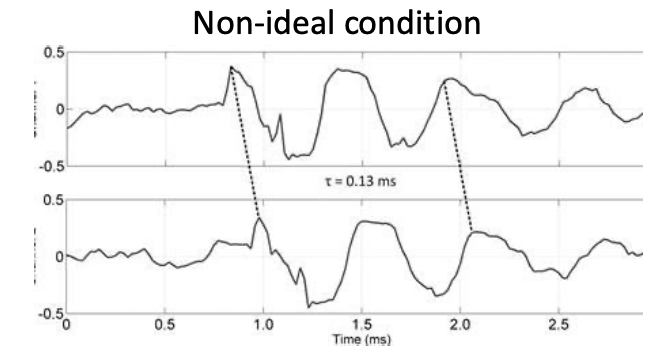
\includegraphics[width=0.4\textwidth]{images/nonideal}
   \caption{Signals under non-ideal condition} \end{figure}
 \item A possible estimate of the delay between the two signals is the time interval by which we need \textbf{to shift one of the signals
   so that it is maximally similar to the other}.
\end{itemize}

 Normalized cross-correlation function between $x_{1}(t)$ and $x_{2}(t)$:
 \begin{align*}\begin{split}
 f_{c}(\theta) &= \frac{\langle x_{1}(t), x_{2}(t-\theta) \rangle}{ \lvert \lvert x_{1}(t) \rvert \rvert_{2} \ \lvert \lvert x_{2}(t) \rvert \rvert_{2}} \\\\
 &= \frac{\int_{-\infty}^{\infty}  x_{1}(t) x_{2}(t-\theta) dt}{\sqrt{\int_{-\infty}^{+\infty}\lvert x_{1}(t)
 \rvert^{2} dt} \cdot \sqrt{\int_{-\infty}^{+\infty}\lvert x_{2}(t-\theta) \rvert^{2} dt}}
 \end{split} \end{align*}
\begin{itemize}
    \item The $\theta$ value corresponding to the maximum of $f(\theta)$ is an estimate of the delay between the two signals.
 \end{itemize}
 
 \begin{ex}{- Measure muscle fiber conduction velocity}
 \begin{minipage}{0.4\textwidth}
 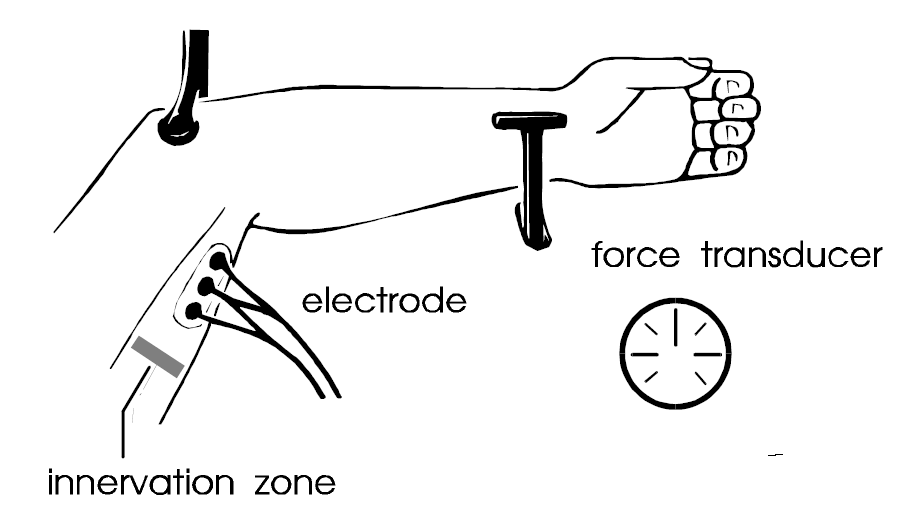
\includegraphics[width=\textwidth]{images/emg3}
 \end{minipage}\hfill
 \begin{minipage}{0.4\textwidth}
 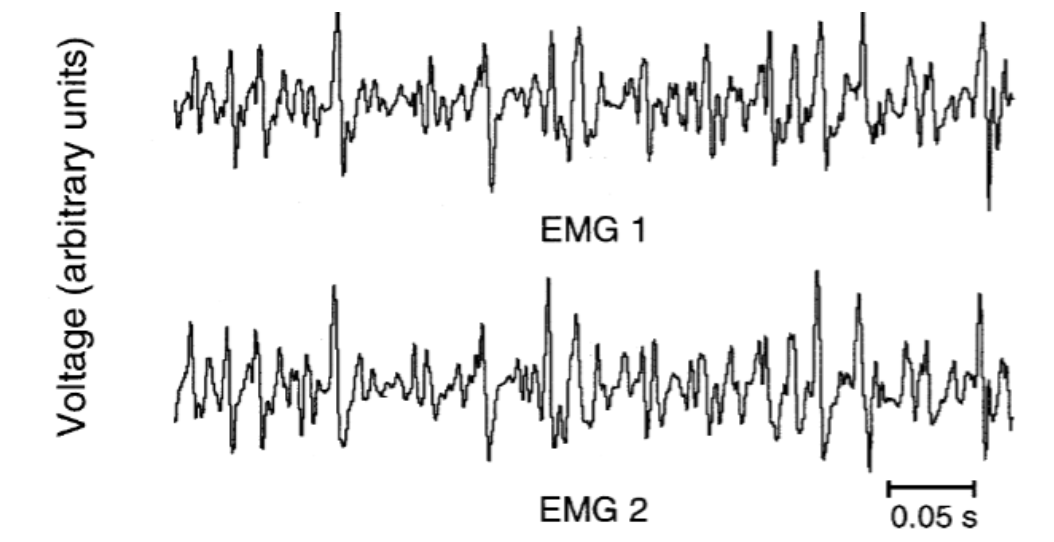
\includegraphics[width=\textwidth]{images/emg1}
 \end{minipage}
\ \\
 By using cross-correlation function, we are able to find the time delay between two EMG signals. By measuring the distance between two electrodes, we can calculate the conduction velocity.
 \begin{figure}[H] \centering
  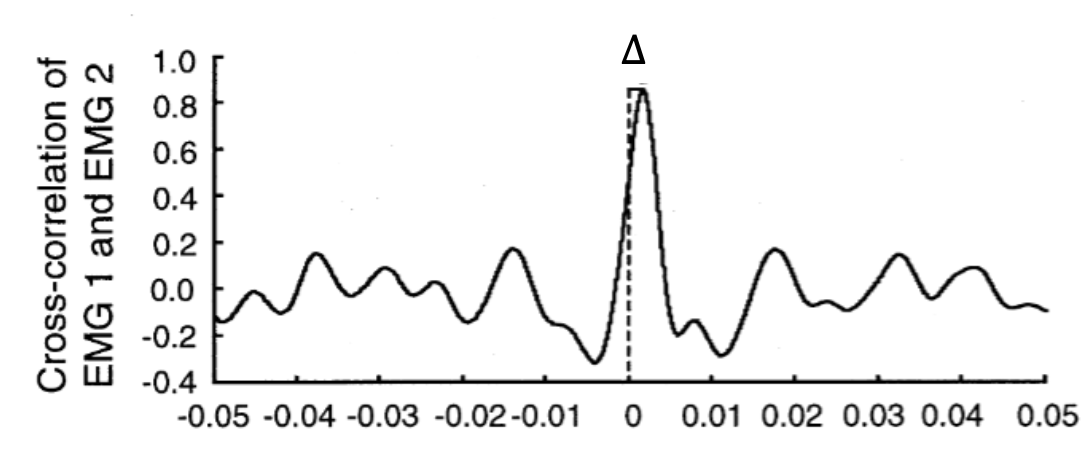
\includegraphics[width=0.5\textwidth]{images/emg2}
\end{figure}
\end{ex}
 
 
\subsubsection{Measuring the Difference}
\begin{itemize}
\item An alternative way to measure the similarity between two signals is to compute the \textbf{strength of their difference} (i.e., norm). 

\item For example, using the norm-2 as measure of strength, we can define the \textbf{mean squared error (MSE)} between signals :
\begin{align*} \begin{split} 
MSE(\theta) &= \lvert \lvert x_{1}(t) - x_{2}(t-\theta) \rvert \rvert_{2}^{2}\\
&=\int_{-\infty}^{+\infty}  \lvert x_{1}(t) - x_{2}(t-\theta) \rvert^{2} dt
\end{split} \end{align*}
\begin{itemize}
\item $MSE(\theta)$ is a function of the shift $\theta$.
\item Minimum value of $\theta$ best estimates the delay. 
\item It is the energy of the error signal.
\end{itemize}
\end{itemize}